\section{实现}
\subsection{数据采集}
职位信息作为招聘网站的核心要素,通常设有保护措施防止被大规模爬取。许多招聘网站
只允许登录用户查看职位信息。但同时,有些网站为了吸引流量,也会开放部分的岗位信息
给未登录用户浏览。在本项目中,我们挑选了两家允许未登录用户浏览职位的网站——\href{liepin.com}{猎聘网}和\href{zhipin.com}{BOSS直聘},用于采集所需要的职位信息。

\subsubsection{猎聘网数据的爬取}
图\ref{liepin}为猎聘的主页。点击位于导航栏的“职位”后,便可以跳转至图\ref{liepinJob}的职位展示页面。

\begin{figure}[!htbp]
    \centering
    
\includegraphics[width=\textwidth]{figures/liepin.png}
    \caption{猎聘主页}\label{liepin}
\end{figure}

\begin{figure}[!htbp]
    \centering
    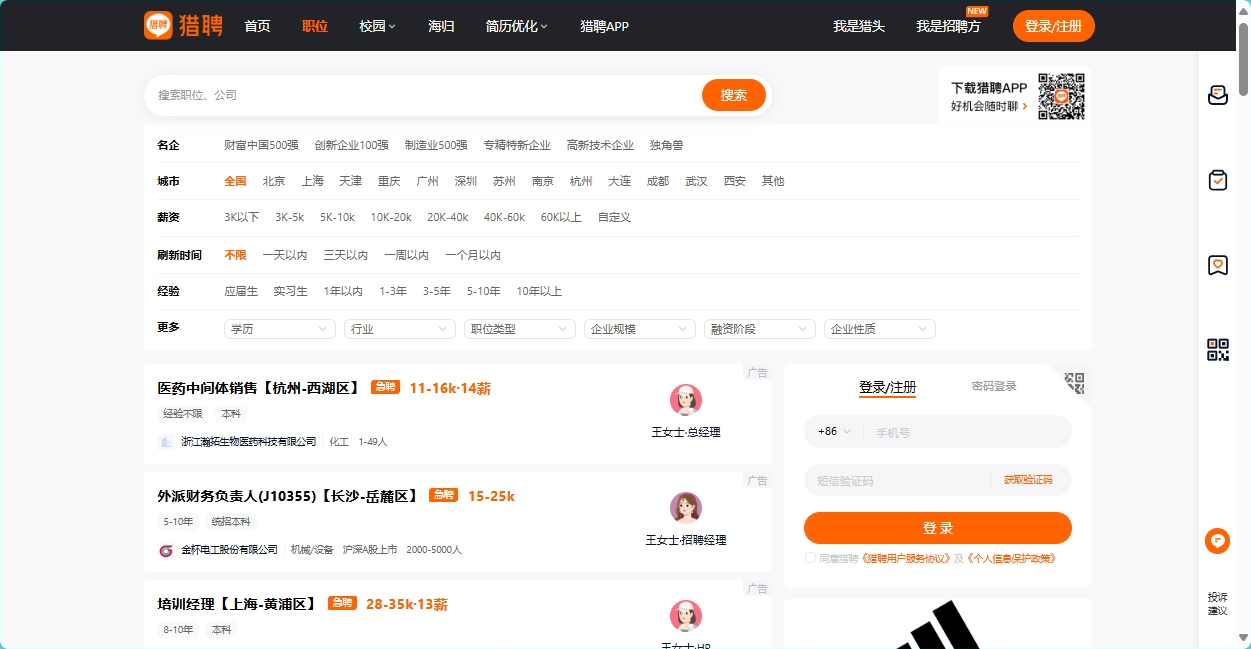
\includegraphics[width=\textwidth]{figures/liepinJob.png}
    \caption{猎聘职位页面}\label{liepinJob}
\end{figure}


如图\ref{response}所示,使用开发者工具查看网络情况,可以看到该页面上的职位信息是通过动态请求的方式获取到的。从图\ref{payload}
可以看出,响应的请求报文的载荷由两部分组成:1)职位的筛选条件;2)passThroughForm。其中,passThroughForm难以模拟,因此我们
放弃使用requests库进行爬取,而是使用selenium库进行后续的爬取。

\begin{figure}[!htbp]
    \centering
    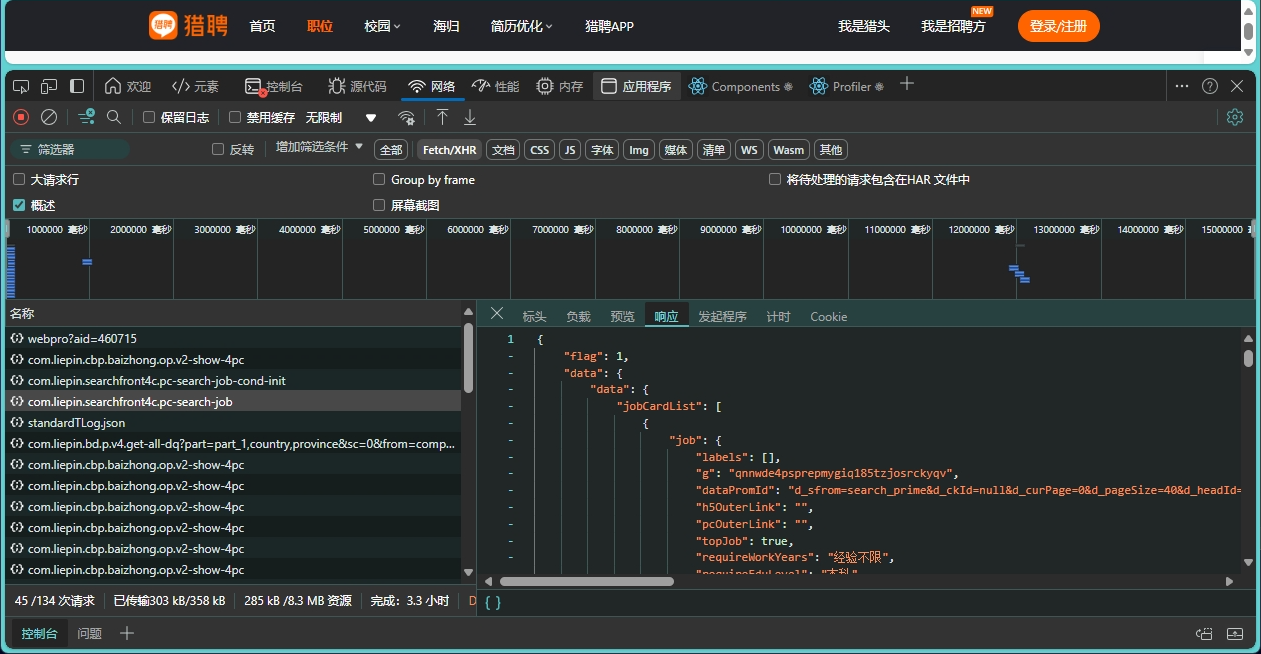
\includegraphics[width=\textwidth]{figures/response.png}
    \caption{含有职位数据的回复报文}\label{response}
\end{figure}

\begin{figure}[!htbp]
    \centering
    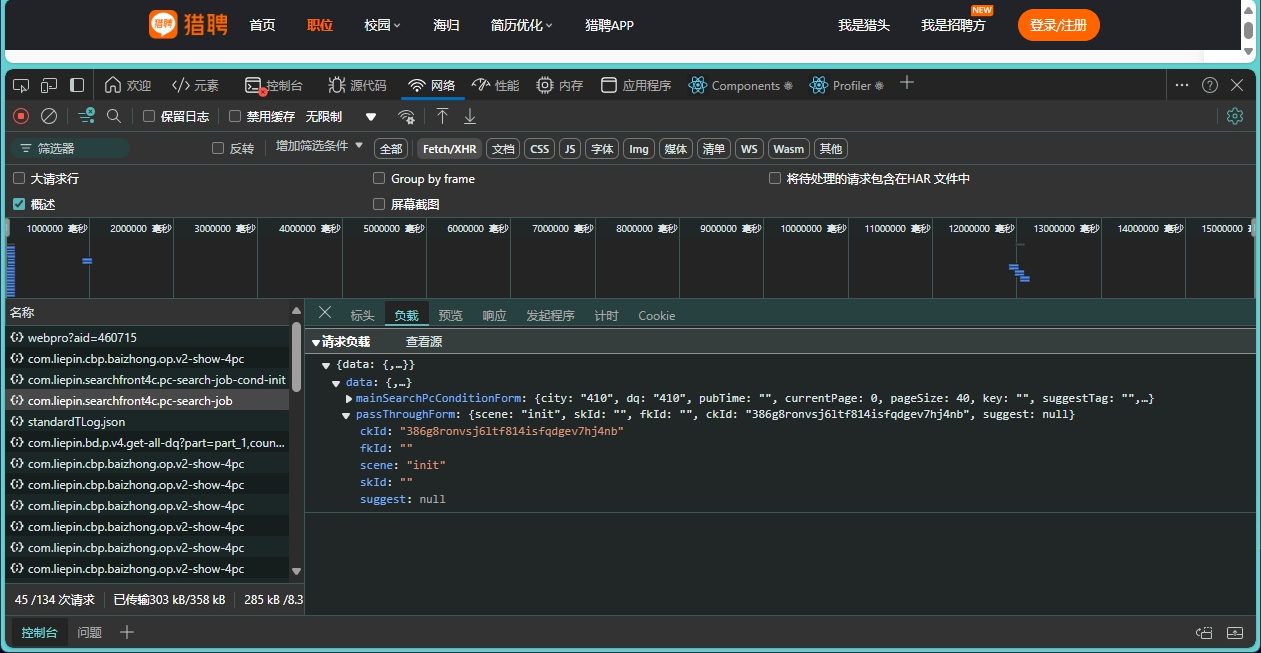
\includegraphics[width=\textwidth]{figures/payload.png}
    \caption{请求职位数据所需载荷}\label{payload}
\end{figure}

由于本项目的主题是“上海市信息类职位分析平台”。所以我们需要在城市筛选条件中选择“上海”,并且
在行业中选择“信息类”。同时,为了尽可能多地采集数据,我们会对“名企”、“薪资”、“经验”这三个条件的所有组合逐一进行爬取。
对于每个条件组合,我们都会创建一个selenium实例。

如图\ref{options}所示,我们可以通过 \texttt{filter-options-row-section}来定位到筛选条件按钮所在区域;根据 \texttt{row-title}中的内容来确定是什么筛选条件;
根据 \texttt{data-name}来定位具体的条件对应元素。



\begin{figure}[!htbp]
    \centering
    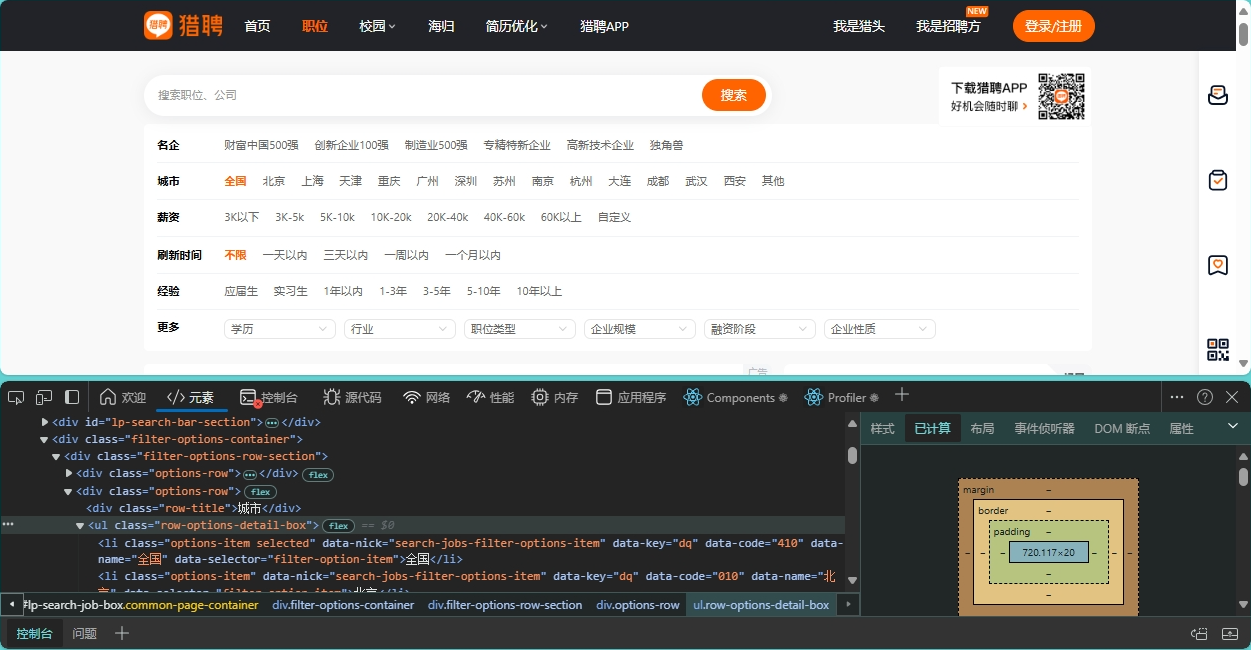
\includegraphics[width=\textwidth]{figures/options.png}
    \caption{职位筛选条件所在元素}\label{options}
\end{figure}

如图\ref{selector}所示,我们可以通过class名中带有 \texttt{select-industries-box}这一条件来定位到条件下拉框对应的元素,这可以通过查找XPATH来实现。

\begin{figure}[!htbp]
    \centering
    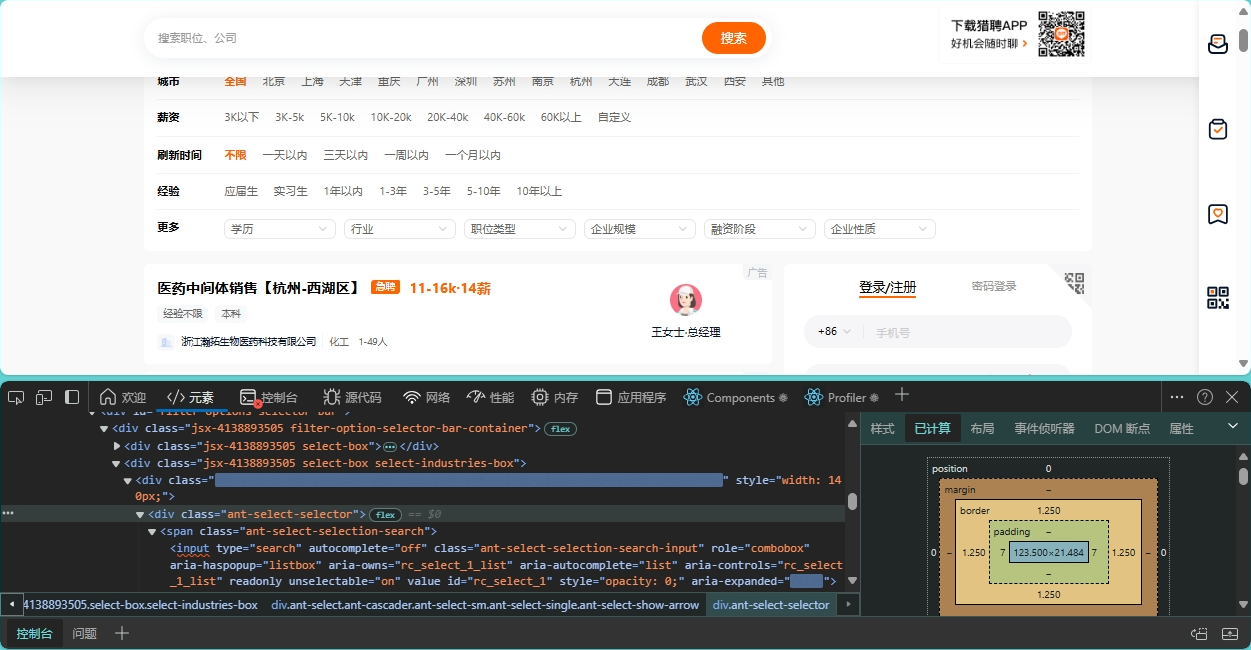
\includegraphics[width=\textwidth]{figures/selector.png}
    \caption{行业筛选条件所在元素}\label{selector}
\end{figure}

如图\ref{card}所示,我们可以通过class名为 \texttt{job-list-box}这一条件来获取各个职位卡片,然后遍历各个卡片,获取其中的职位信息。

\begin{figure}[!htbp]
    \centering
    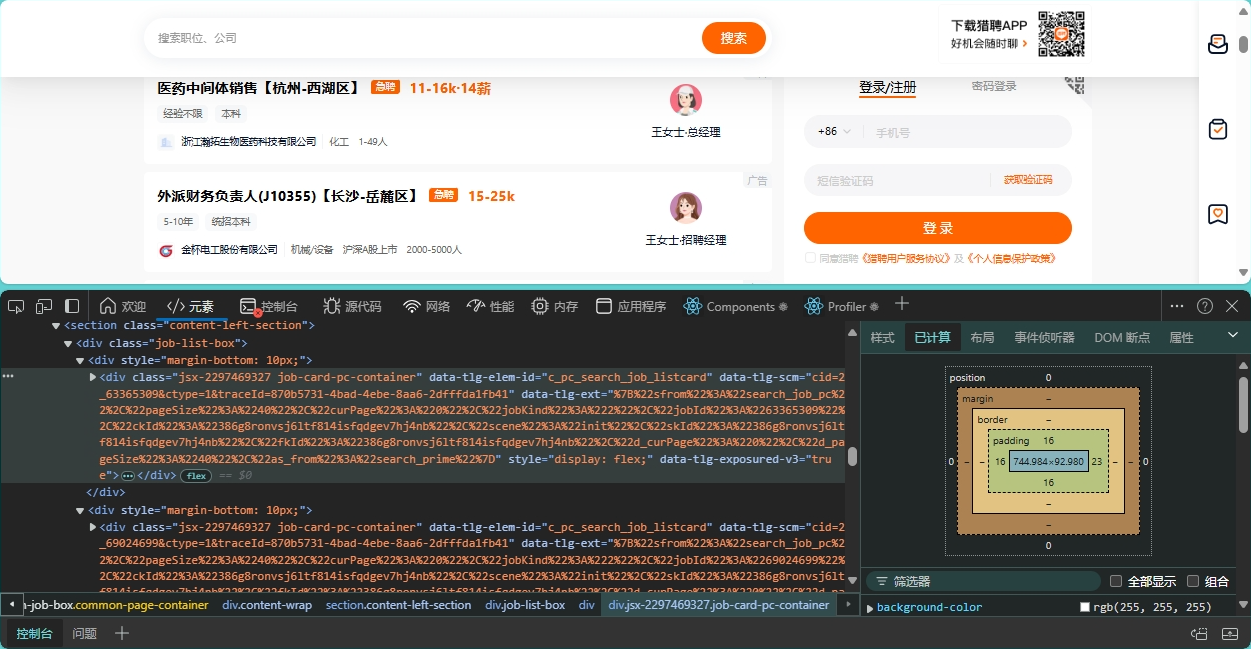
\includegraphics[width=\textwidth]{figures/card.png}
    \caption{职位信息所在元素}\label{card}
\end{figure}

如图\ref{nextpage}所示,我们可以通过 title对于 Next Page这一条件来定位到切换至下一页的按钮所在元素。可以通过该元素是否有效来判断是否已经是最后一页。

\begin{figure}[!htbp]
    \centering
    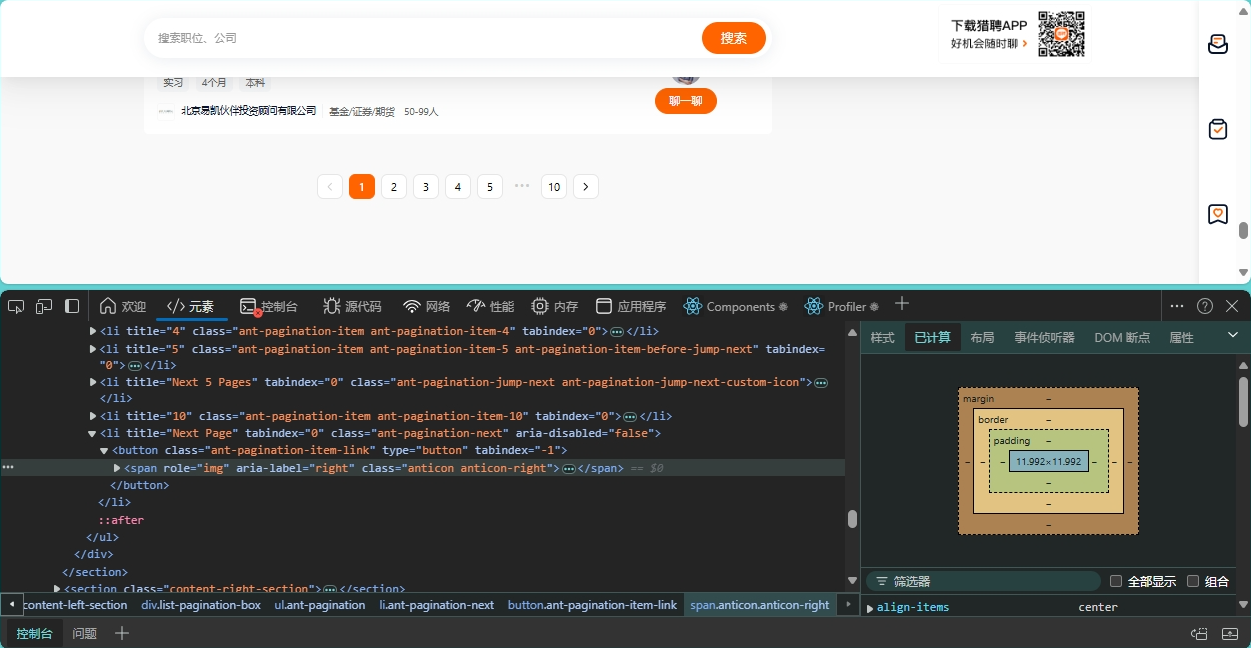
\includegraphics[width=\textwidth]{figures/nextpage.png}
    \caption{翻页按钮所在元素}\label{nextpage}
\end{figure}

在实际采集的过程中,经常会出现跳出如图\ref{login}所示的登录页的情况。为此,我们使用\href{www.qg.net}{青果网络}的隧道代理服务,每次创建一个selenium实例便更换一次IP地址。
同时,我们通过异常捕获机制允许对同一条件尝试10次,若失败次数到达10次,则记录到错误日志中,可以后续集中重新爬取。为了模拟人类行为,我们在每次操作之间增加了服从高斯分布的睡眠时间。

\begin{figure}[!htbp]
    \centering
    
\includegraphics[width=\textwidth]{figures/login.png}
    \caption{登录页}\label{login}
\end{figure}

在爬取的过程中,我们同步将获得的数据写入SQLite数据库。整个爬取过程用时约14个小时,共爬取近6000条数据。有15个条件组合爬取失败。

\subsubsection{BOSS直聘数据的爬取}

图\ref{BOSS}为BOSS直聘的首页。点击导航栏中的“搜索”,既可以跳转至图\ref{BOSSJob}中的职位搜索页,能够满足我们项目对于岗位的筛选需求。
该搜索网页的url为\texttt{https://www.zhipin.com/web/geek/job?query=},选择若干筛选条件后,可以看到url的变化仅为添加了相应的参数。例如,
在城市中选择“天津”,然后在区域中选择“西青区(全)”,再选择Java岗位类型,并限制为全职后,url变为\texttt{https://www.zhipin.com/web/geek/job?city=101030100\\\&position=100101\&jobType=1901\&areaBusiness=120111},
各参数的含义明确。因此我们首先尝试使用requests库,通过构造url的方式来进行爬取。经过尝试,我们发现必须要使用cookie才能成功申请到数据。
由于本项目所需采集的数据量较大,因此我们决定使用selenium进行爬取,避免了手动提取cookie的步骤。

与爬取猎聘网的过程不同,由于BOSS直聘的url容易模拟,我们可以直接通过selenium实例的get方法来直接设置所有的筛选条件,而无需通过通过模拟逐个点击筛选条件的方式。
这使得爬取BOSS直聘数据的速度较快,并且由于减少了与网页交互的次数,也更不容易被反爬虫技术所识别。

\begin{figure}[!htbp]
    \centering
    
\includegraphics[width=\textwidth]{figures/BOSS}
    \caption{BOSS直聘主页}\label{BOSS}
\end{figure}

\begin{figure}[!htbp]
    \centering
    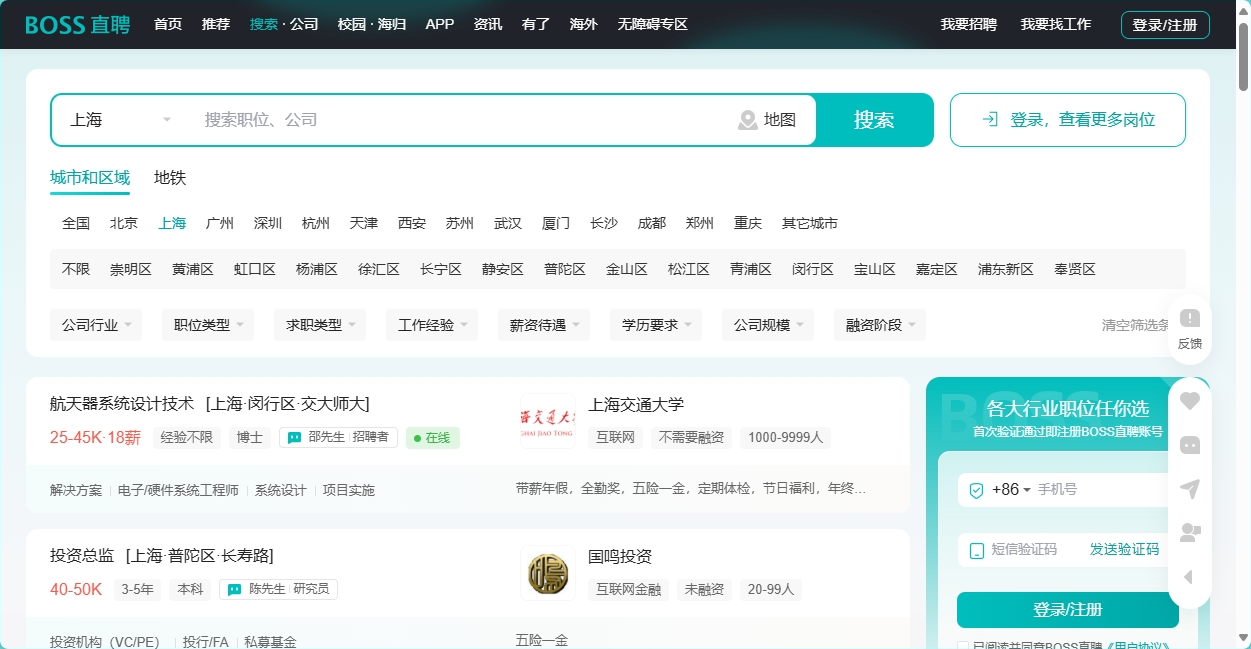
\includegraphics[width=\textwidth]{figures/BOSSJob.png}
    \caption{BOSS直聘搜索页面}\label{BOSSJob}
\end{figure}

如图\ref{wrapper}所示,我们可以通过class为\texttt{job-card-wrapper}这一条件来获取所有的工作卡片,从而进一步逐一从中提取岗位的具体信息。


\begin{figure}[!htbp]
    \centering
    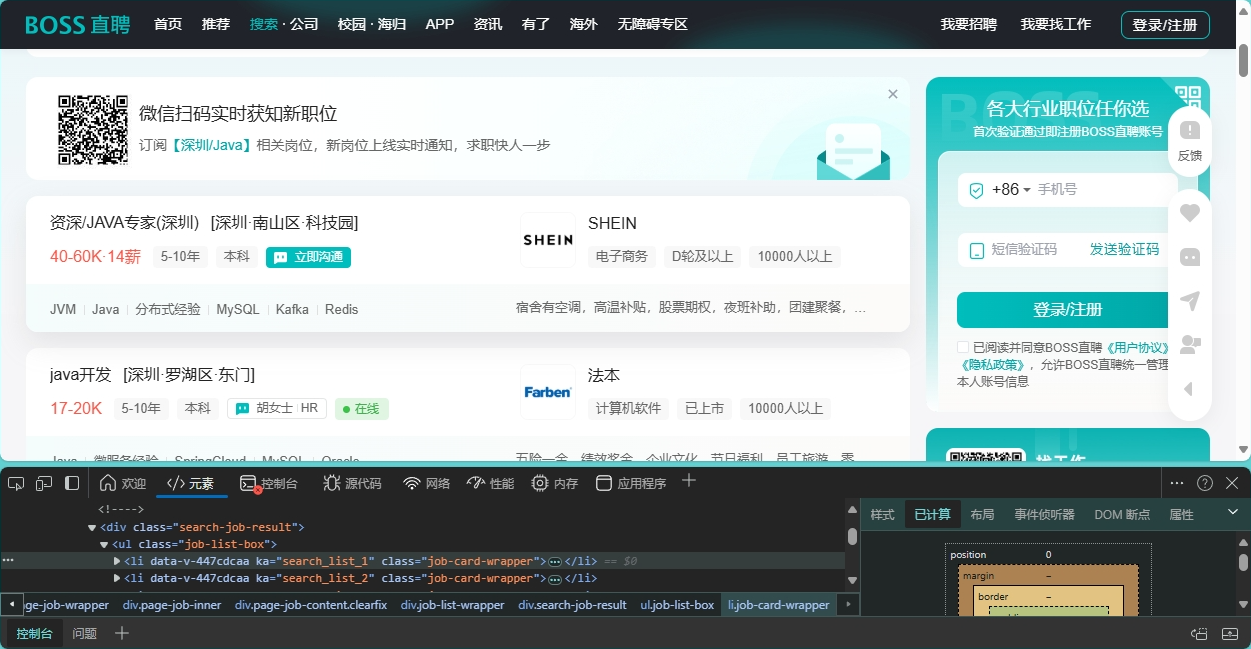
\includegraphics[width=\textwidth]{figures/wrapper.png}
    \caption{定位工作信息所在元素}\label{wrapper}
\end{figure}

如图\ref{next}所示,我们可以通过class为\texttt{ui-icon-arrow-right}这一条件来定位到翻页按钮所在元素。我们可以通过该元素是否启用来判断是否以及到达最后一页。
为了防止被识别为爬虫程序,我们采用\verb|ActionChains|类来模拟人类的行为。

\begin{figure}[!htbp]
    \centering
    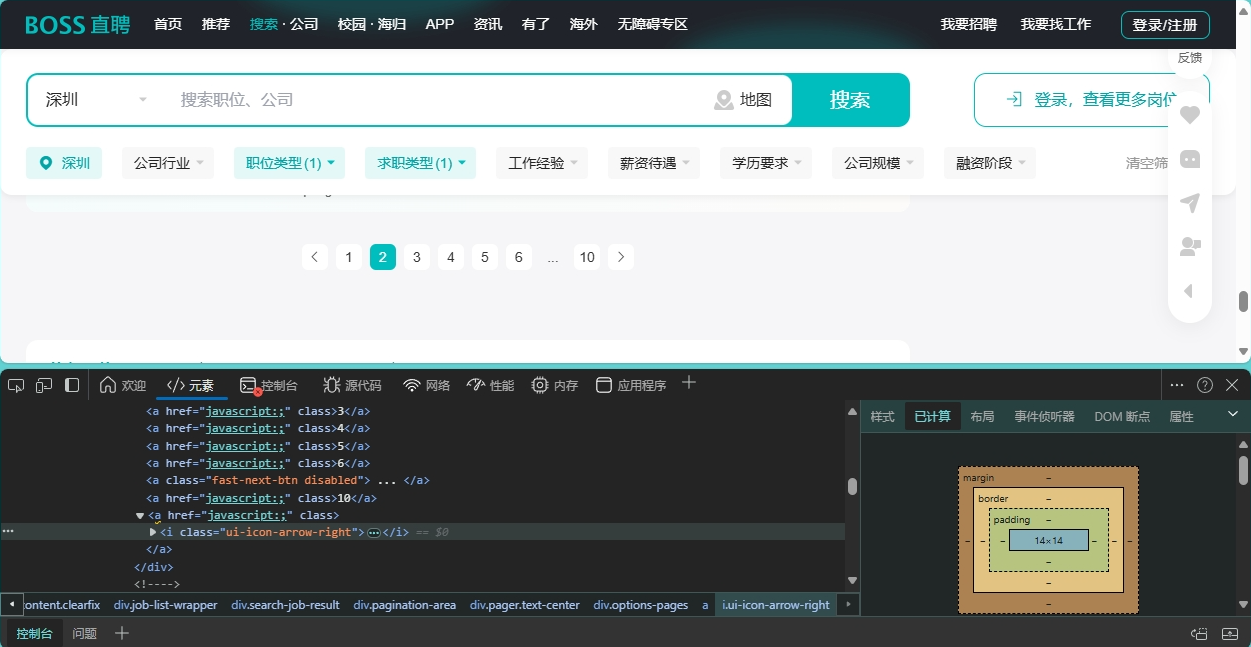
\includegraphics[width=\textwidth]{figures/next.png}
    \caption{翻页按钮所在元素}\label{next}
\end{figure}

\subsubsection{58招聘数据的爬取}

在数据采集的过程中,我们也尝试爬取58招聘网站的数据。图\ref{58}为58招聘网站的主页,点击导航栏中的社会招聘,将跳转至
图\ref{58job}中的岗位详情页面。

\begin{figure}[!htbp]
    \centering
    
\includegraphics[width=\textwidth]{figures/58.png}
    \caption{58招聘主页}\label{58}
\end{figure}

\begin{figure}[!htbp]
    \centering
    
\includegraphics[width=\textwidth]{figures/58job.png}
    \caption{58招聘岗位页面}\label{58job}
\end{figure}

如图\ref{58network}所示,通过开发者工具查看网络活动情况,我们发现该网页的岗位数据是通过动态请求的方式获取的,
相应的载荷如图\ref{58payload}所示。并且,通过开发者工具我们可以看到该请求的请求标头中不含有cookie。因此我们直接通过
requests库来获取。

\begin{figure}[!htbp]
    \centering
    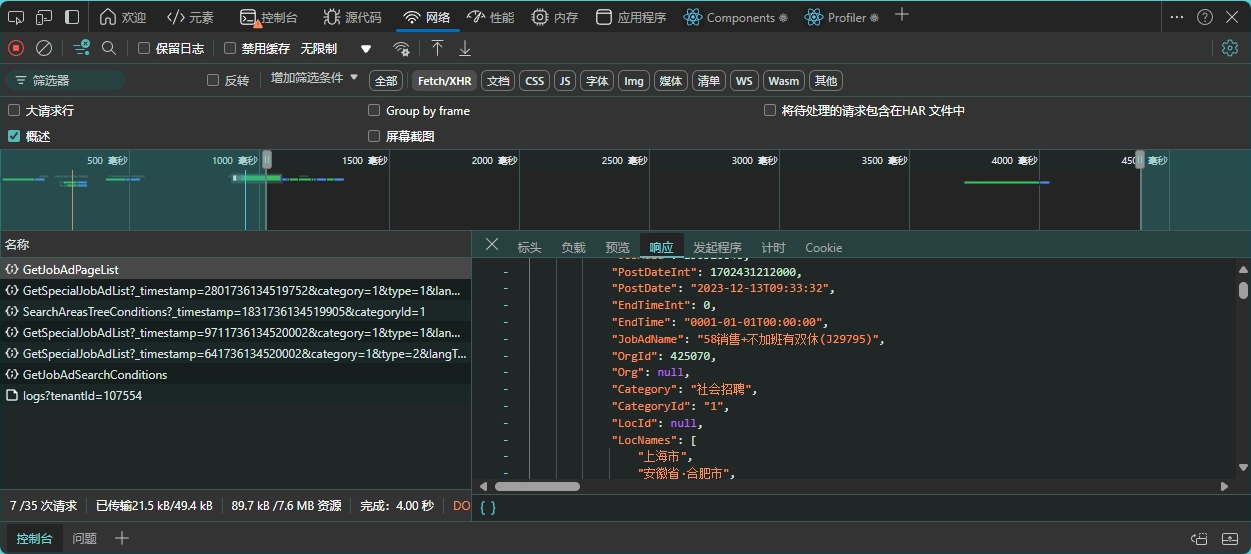
\includegraphics[width=\textwidth]{figures/58network.png}
    \caption{58招聘岗位页面网络请求情况}\label{58network}
\end{figure}

\begin{figure}[!htbp]
    \centering
    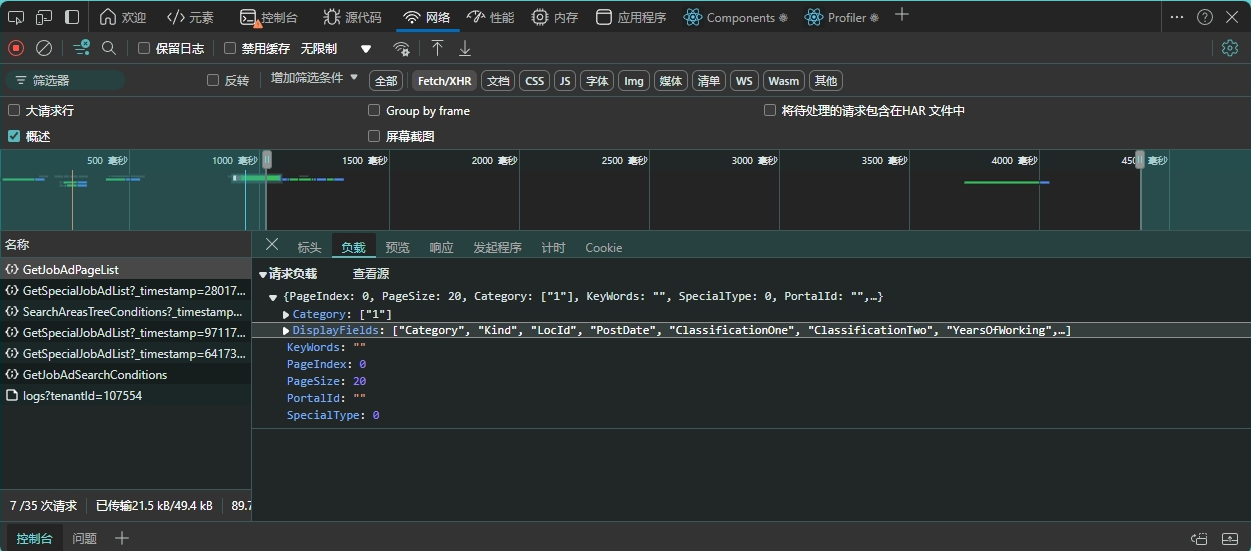
\includegraphics[width=\textwidth]{figures/58payload.png}
    \caption{58招聘岗位信息请求所需负载}\label{58payload}
\end{figure}

一条典型的工作岗位数如图\ref{data}所示。可以看到,该网站所返回的字段有大量的缺失值,例如\texttt{Salary},\texttt{Degree},\texttt{YearOfWorking}等。
这些信息都被集中在\texttt{Duty},\texttt{Require}字段中。
同时,我们发现58招聘网站上发布的岗位信息与先前爬取的猎聘网和BOSS直聘网的岗位数据有较大不同。例如58招聘网中的岗位信息中不包含公司名称,
薪资大多是“面谈”。上述这些特点都给后续的数据集成阶段带来较多不便,因此,在数据集成阶段,我们只采用猎聘网和BOSS直聘网的数据。

\begin{figure}[!htbp]
    \centering
    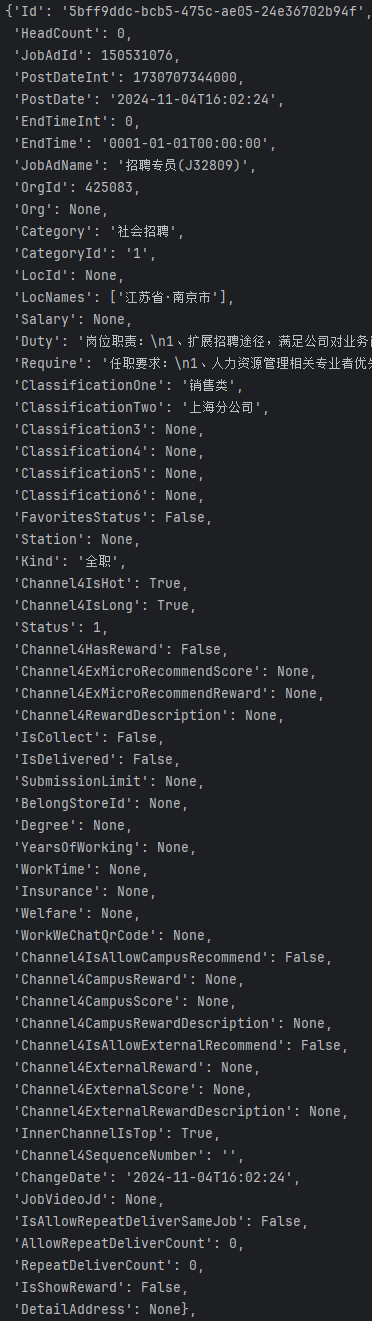
\includegraphics[height=0.8\textheight]{figures/data.png}
    \caption{58招聘岗位数据示例}\label{data}
\end{figure}


\subsection{数据集成}
本系统实现了一个完整的ETL(Extract-Transform-Load)数据集成流程,将来自不同招聘网站的职位数据进行整合、清洗和标准化,最终加载到规范化的数据库中。整个过程包括数据抽取(Extract)、数据转换(Transform)和数据加载(Load)三个主要阶段。如图\ref{fig:ETL}所示。

\begin{figure}[htbp]
    \centering
    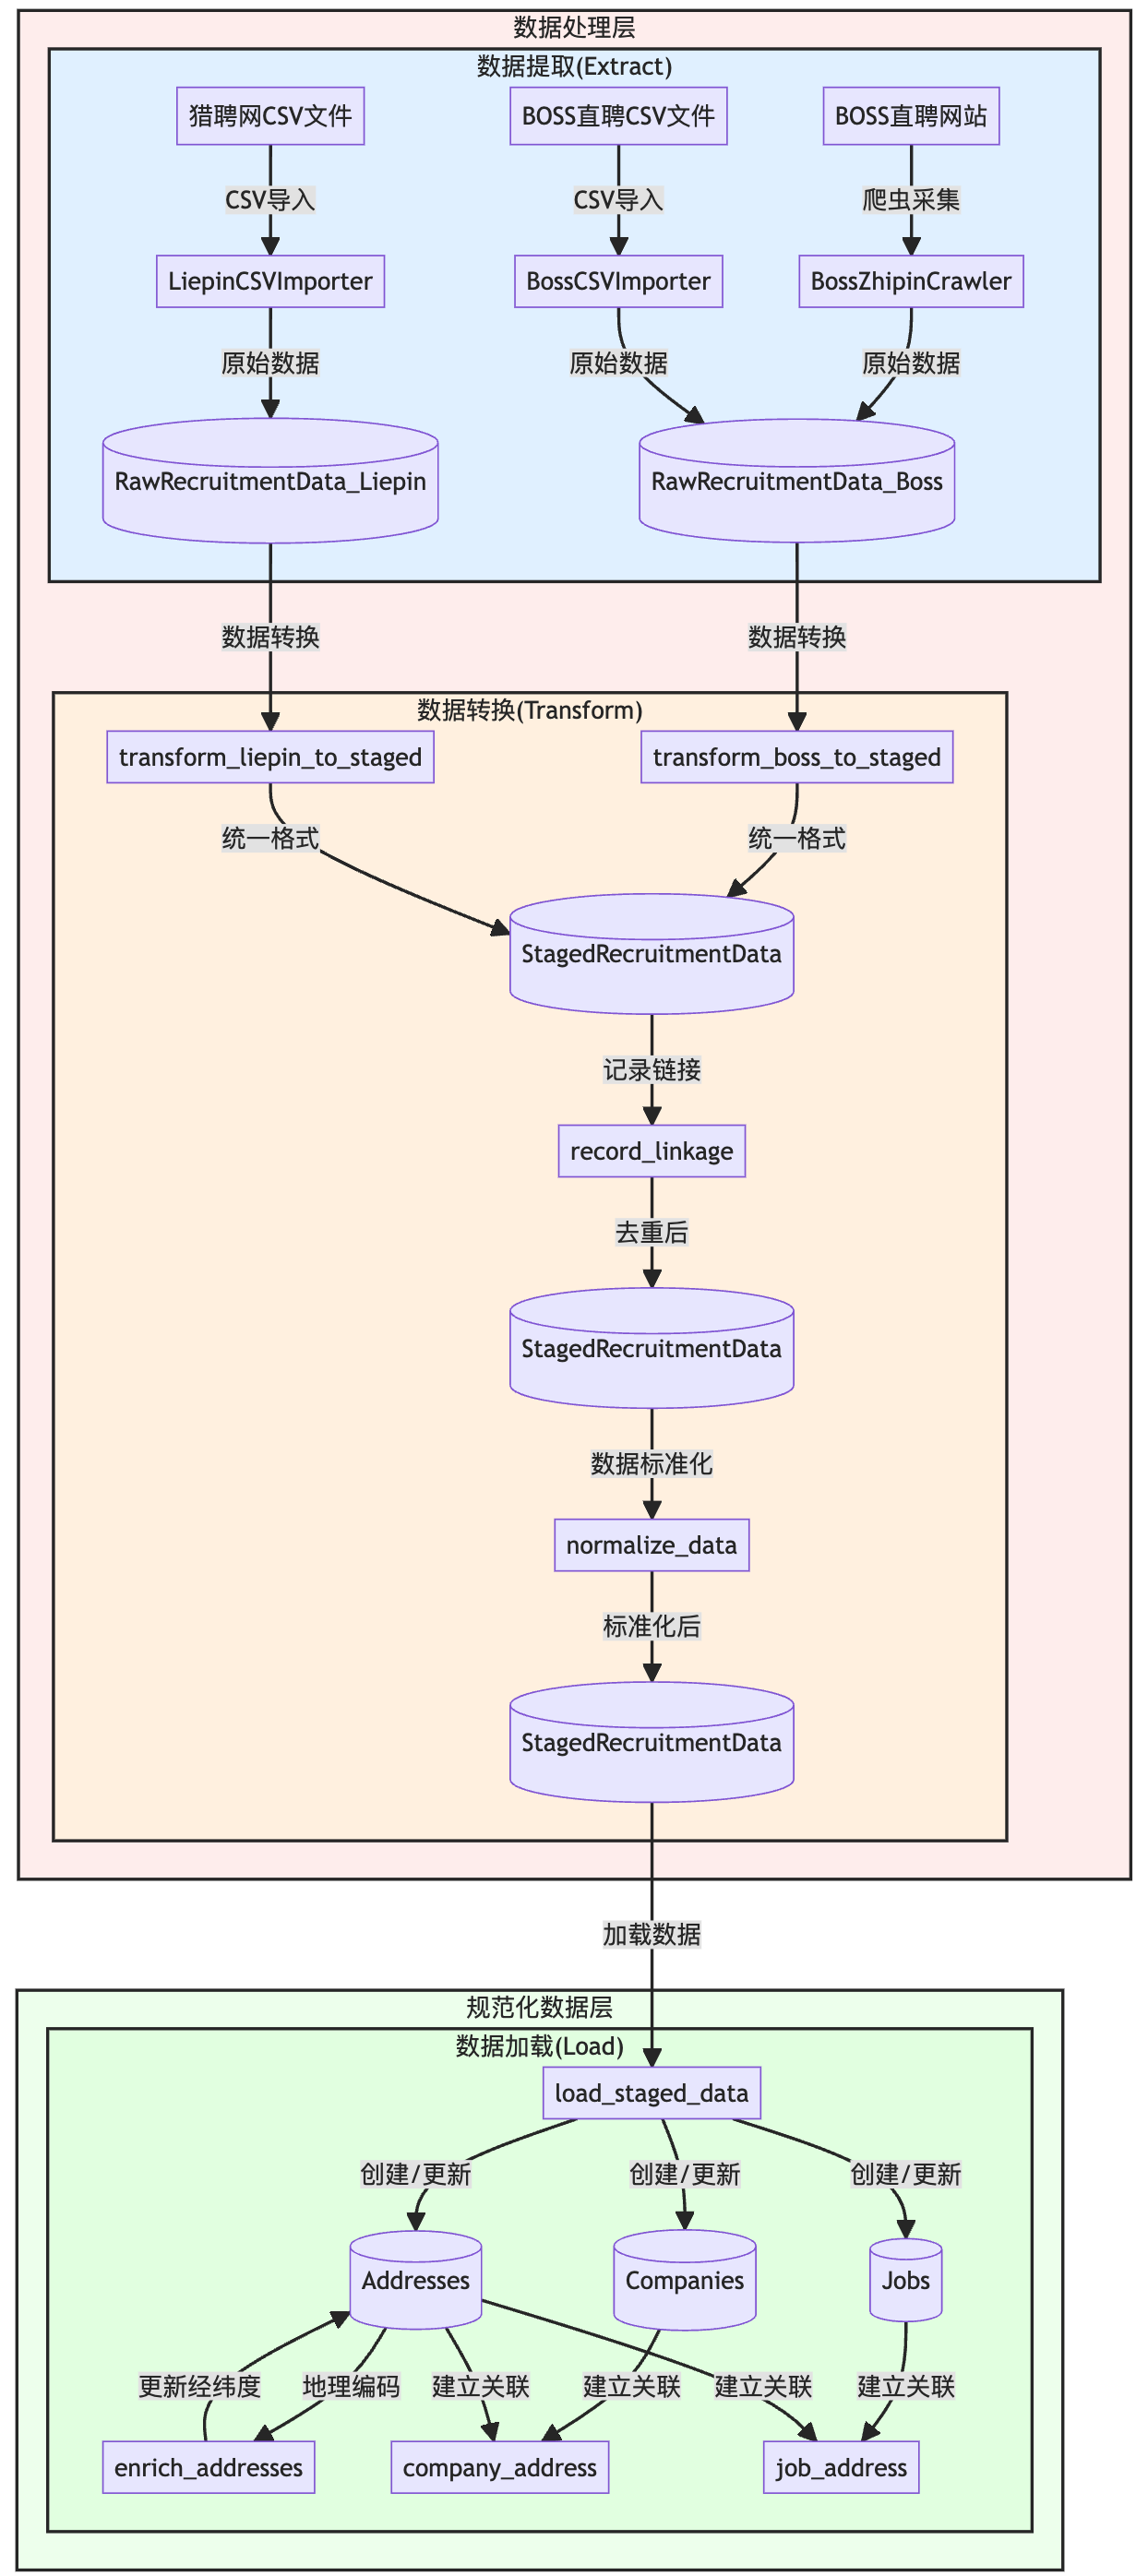
\includegraphics[width=0.6\textwidth]{figures/ETL.png}
    \caption{ETL数据集成流程}
    \label{fig:ETL}
\end{figure}

\subsubsection{数据抽取(Extract)}
数据抽取阶段主要通过两种方式获取数据,如图\ref{fig:ETL_extract}所示。包含下面两个步骤:

\begin{figure}[htbp]
    \centering
    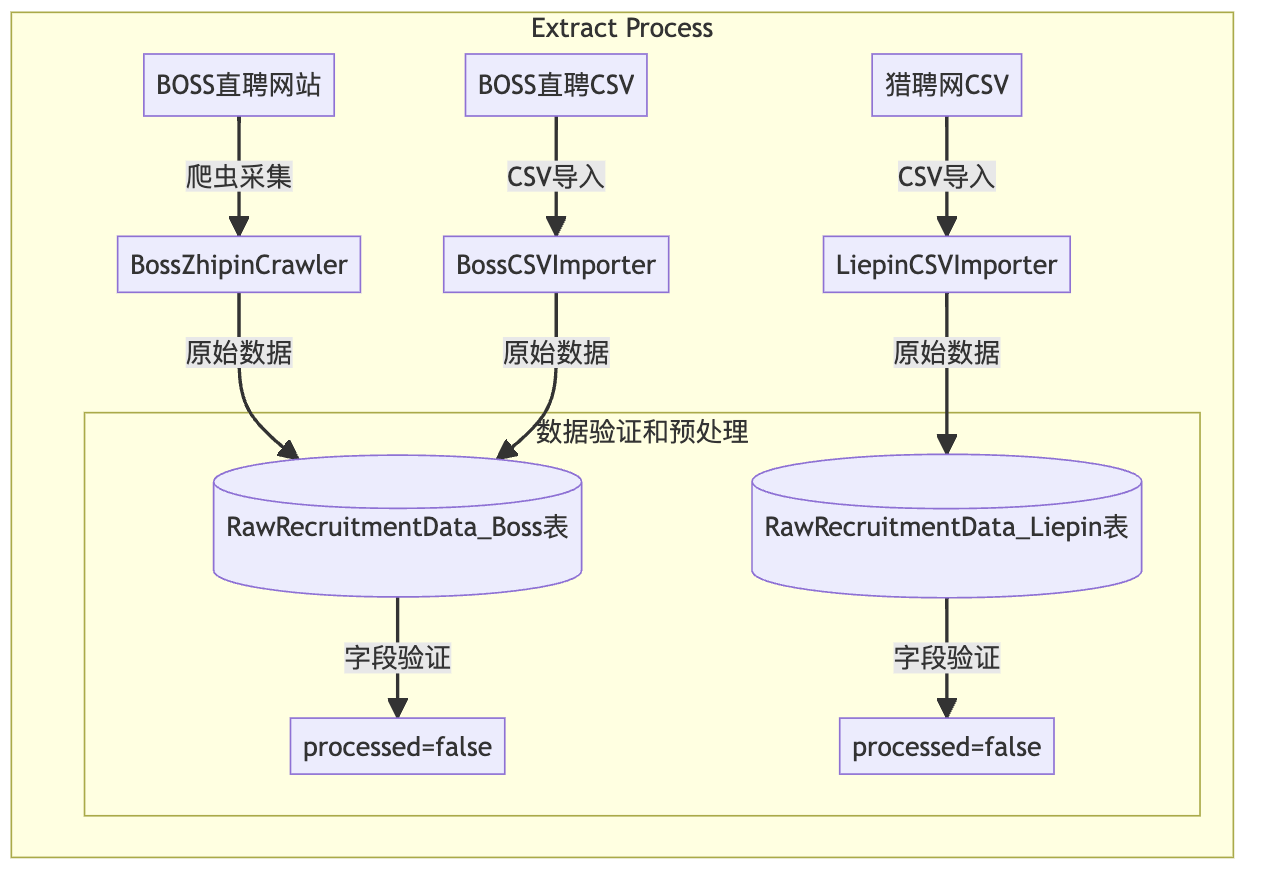
\includegraphics[width=0.5\textwidth]{figures/extract.png}
    \caption{数据抽取流程}
    \label{fig:ETL_extract}
\end{figure}


\begin{itemize}
    \item \textbf{Boss直聘数据抽取}:
    \begin{itemize}
        \item 使用Selenium实现网页爬虫,支持自动翻页和错误重试
        \item 提取职位信息、公司信息、地址等数据
        \item 数据直接存入raw\_recruitment\_boss表
    \end{itemize}
    
    \item \textbf{猎聘网数据导入}:
    \begin{itemize}
        \item 通过CSV文件导入,支持批量处理和数据验证
        \item 数据存入raw\_recruitment\_liepin表
    \end{itemize}
\end{itemize}

\subsubsection{数据转换(Transform)}
数据转换阶段是整个ETL过程中最复杂的部分,主要包括以下几个关键步骤,如图\ref{fig:ETL_transform}所示。

\begin{figure}[htbp]
    \centering
    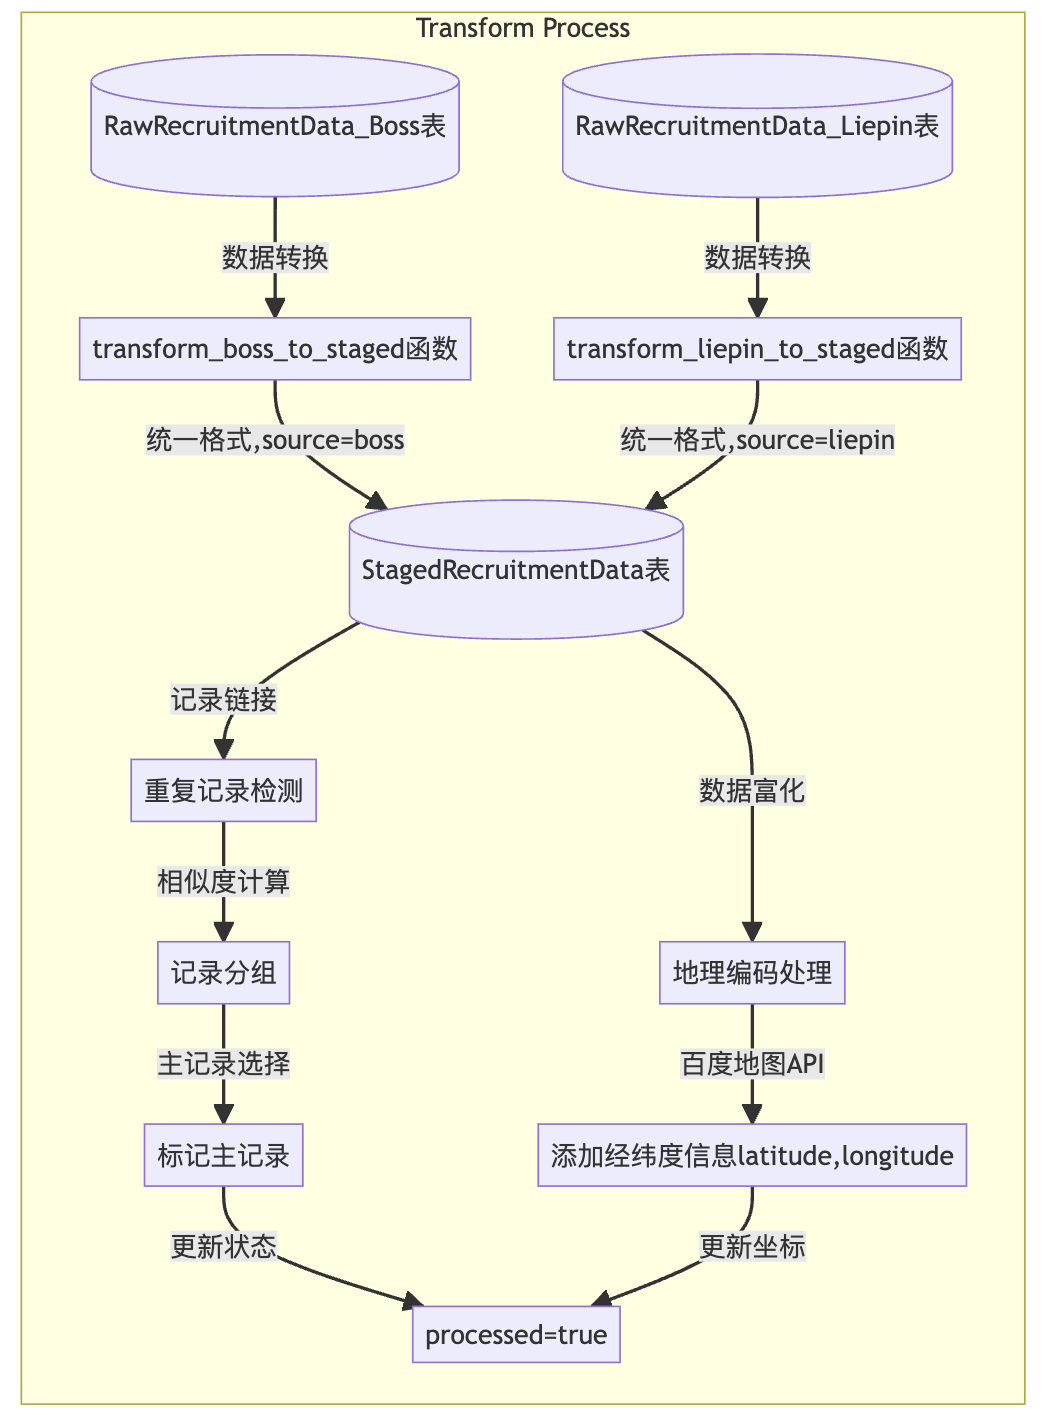
\includegraphics[width=0.5\textwidth]{figures/transform.png}
    \caption{数据转换流程}
    \label{fig:ETL_transform}
\end{figure}

数据转换过程主要包括三个部分:Boss直聘数据转换、猎聘网数据转换以及额外字段转换。如图\ref{fig:boss_transform}、图\ref{fig:liepin_transform}和图\ref{fig:extra_transform}所示。

\begin{figure}[htbp]
    \centering
    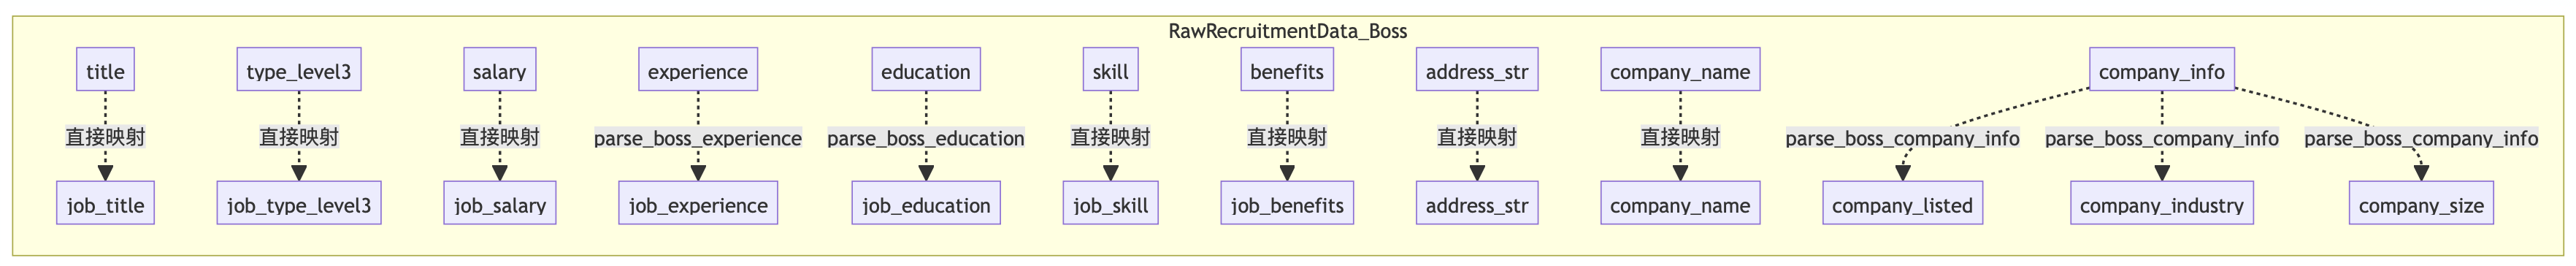
\includegraphics[width=1.0\textwidth]{figures/T过程boss.png}
    \caption{Boss直聘数据转换流程}
    \label{fig:boss_transform}
\end{figure}

从图\ref{fig:boss_transform}可以看出,Boss直聘数据的转换过程主要包括直接映射和解析转换两种方式。其中title、type\_level3、salary等字段可以直接映射到目标表,而experience、education和company\_info等字段则需要通过特定的解析函数进行转换。

\begin{figure}[htbp]
    \centering
    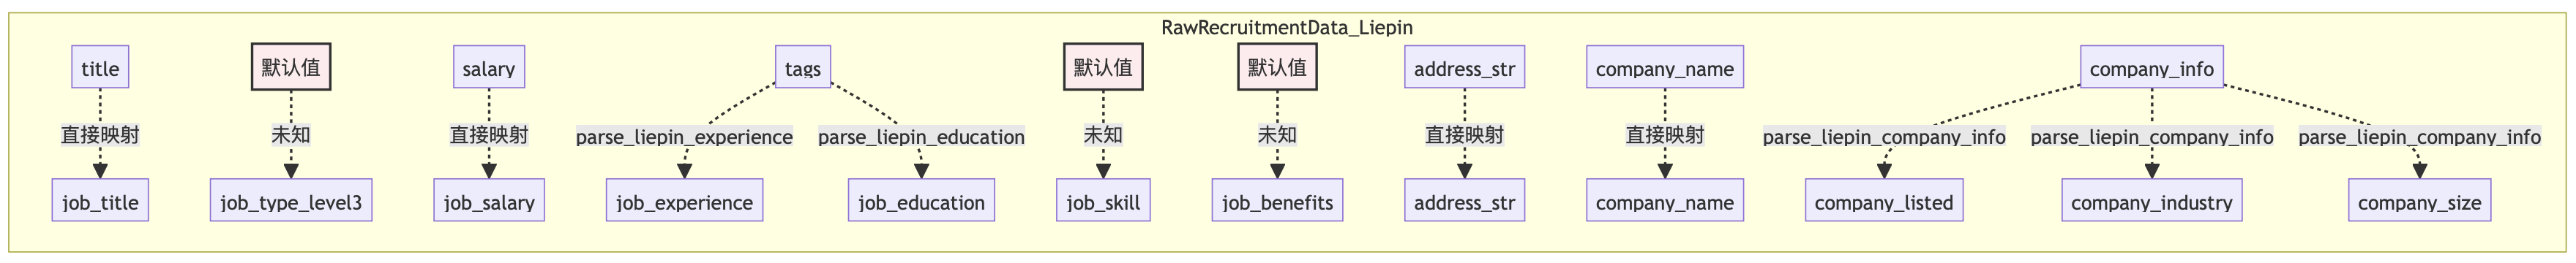
\includegraphics[width=1.0\textwidth]{figures/T过程liepin.png}
    \caption{猎聘网数据转换流程}
    \label{fig:liepin_transform}
\end{figure}

图\ref{fig:liepin_transform}展示了猎聘网数据的转换流程。由于猎聘网的数据结构与Boss直聘不同,需要针对其特有的tags字段进行解析,从中提取职位类型、工作经验、教育要求等信息。

\begin{figure}[htbp]
    \centering
    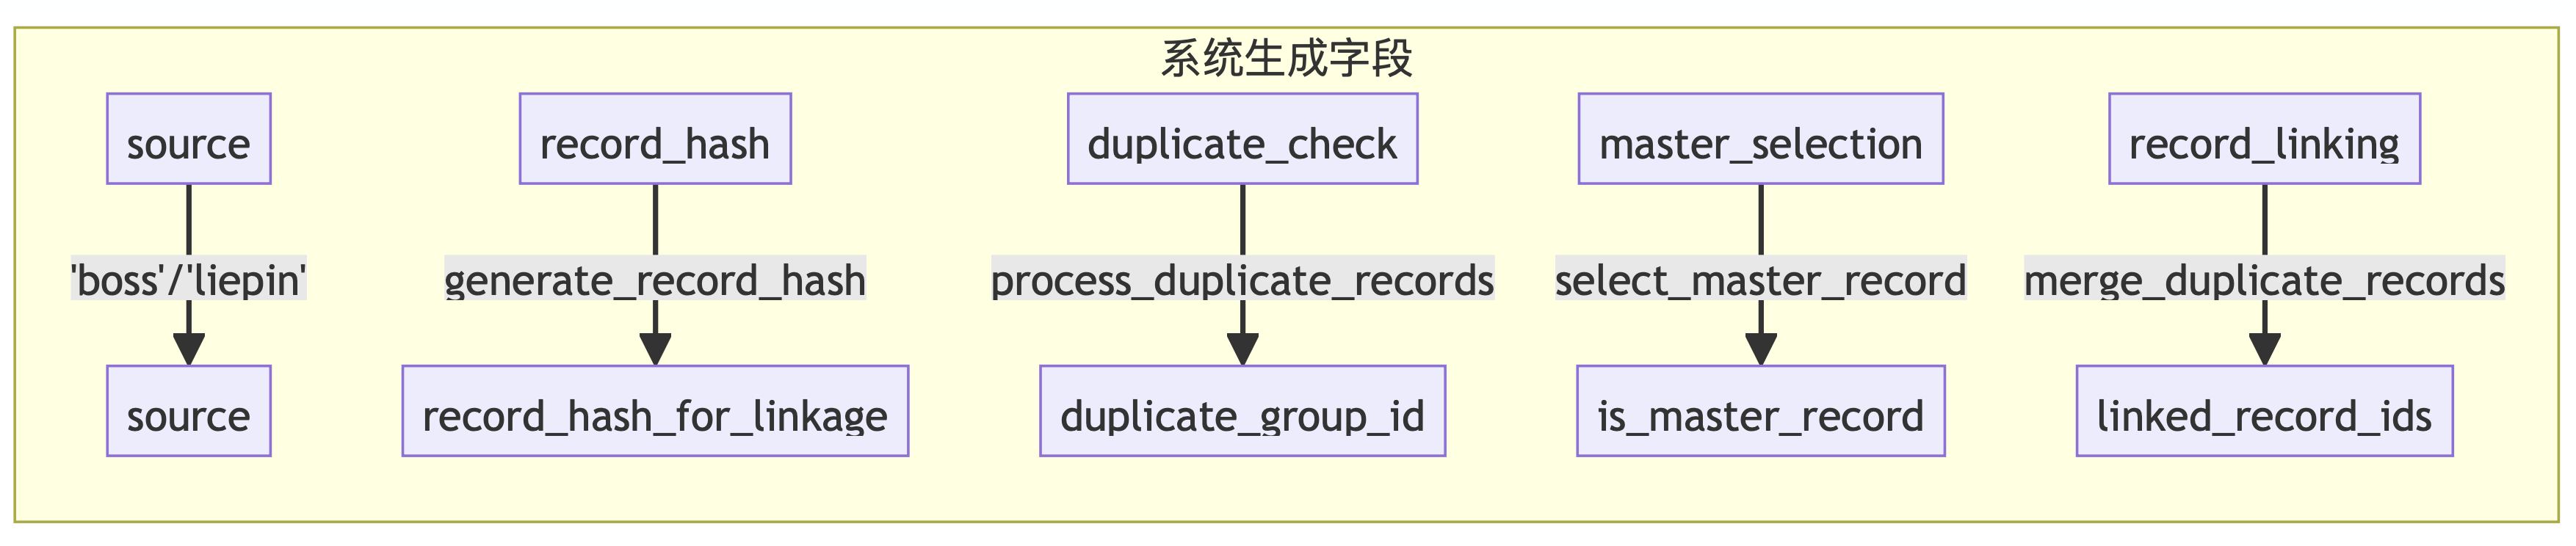
\includegraphics[width=1\textwidth]{figures/T过程extra.png}
    \caption{额外字段转换流程}
    \label{fig:extra_transform}
\end{figure}

图\ref{fig:extra_transform}显示了一些需要额外处理的字段转换过程,包括record\_hash\_for\_linkage的生成、duplicate\_group\_id的分配以及is\_master\_record的判定等。这些字段主要用于后续的记录链接和去重处理。

这个过程可以总结如下:

\begin{itemize}
    \item \textbf{数据清洗和标准化}:
    \begin{itemize}
        \item 实现了文本预处理和标准化
        \item 去除空白字符、转换英文字符为小写
        \item 移除标点符号,保留中文和英文字符
    \end{itemize}
    
    \item \textbf{记录链接和去重}:
    \begin{itemize}
        \item 采用多阶段策略进行记录链接
        \item 使用特征提取和哈希生成进行快速初筛
        \item 通过Jaccard相似度算法计算文本相似度
        \item 动态权重分配,重点关注公司名称和职位名称
    \end{itemize}
    
    \item \textbf{数据融合策略}:
    \begin{itemize}
        \item 智能选择主记录(基于记录完整度)
        \item 维护重复记录之间的关联关系
        \item 支持增量更新和批量处理
    \end{itemize}
\end{itemize}

\subsubsection{数据加载(Load)}

数据加载阶段是ETL过程的最后一个环节,负责将暂存表中的数据规范化加载到最终的数据库中。在这个阶段,系统首先会对数据进行全面的验证和预处理,包括检查必要字段的完整性、验证数据格式的正确性,以及进行必要的数据类型转换。这一步骤确保了进入最终数据库的数据都是高质量且格式统一的。

在数据验证完成后,系统会进行地理编码处理。这个过程通过调用百度地图API,将地址字符串转换为具体的经纬度坐标。系统采用了批量处理的方式提高效率,同时实现了错误重试机制以提高地理编码的成功率。对于无法成功编码的地址,系统会记录详细的错误信息,便于后续人工处理或重试。

最后是数据的规范化加载过程。这个阶段系统会根据数据库的规范化设计,将数据分别加载到不同的实体表中。首先是创建或更新公司信息,系统会检查公司是否已存在,如果存在则更新相关信息,如果不存在则创建新的公司记录。然后是处理地址信息,由于一个公司可能有多个地址,系统支持多地址的处理和存储。接着是创建职位记录,将职位相关的所有信息存入职位表中。最后,系统会建立各个实体之间的关联关系,包括公司与地址之间的关系、职位与地址之间的关系等。整个加载过程采用事务管理机制,确保数据的一致性和完整性。

为了提高数据加载的效率,系统采用了批量处理的策略,同时实现了完善的错误处理机制。当加载过程中出现异常时,系统会自动回滚事务,确保数据库的一致性不被破坏。同时,系统会详细记录每一步的处理结果,包括成功加载的记录数、失败的记录数以及具体的错误原因,这些信息对于后续的数据质量分析和系统优化都有重要的参考价值。

整个过程如图\ref{fig:ETL_load}所示。

\begin{figure}[htbp]
    \centering
    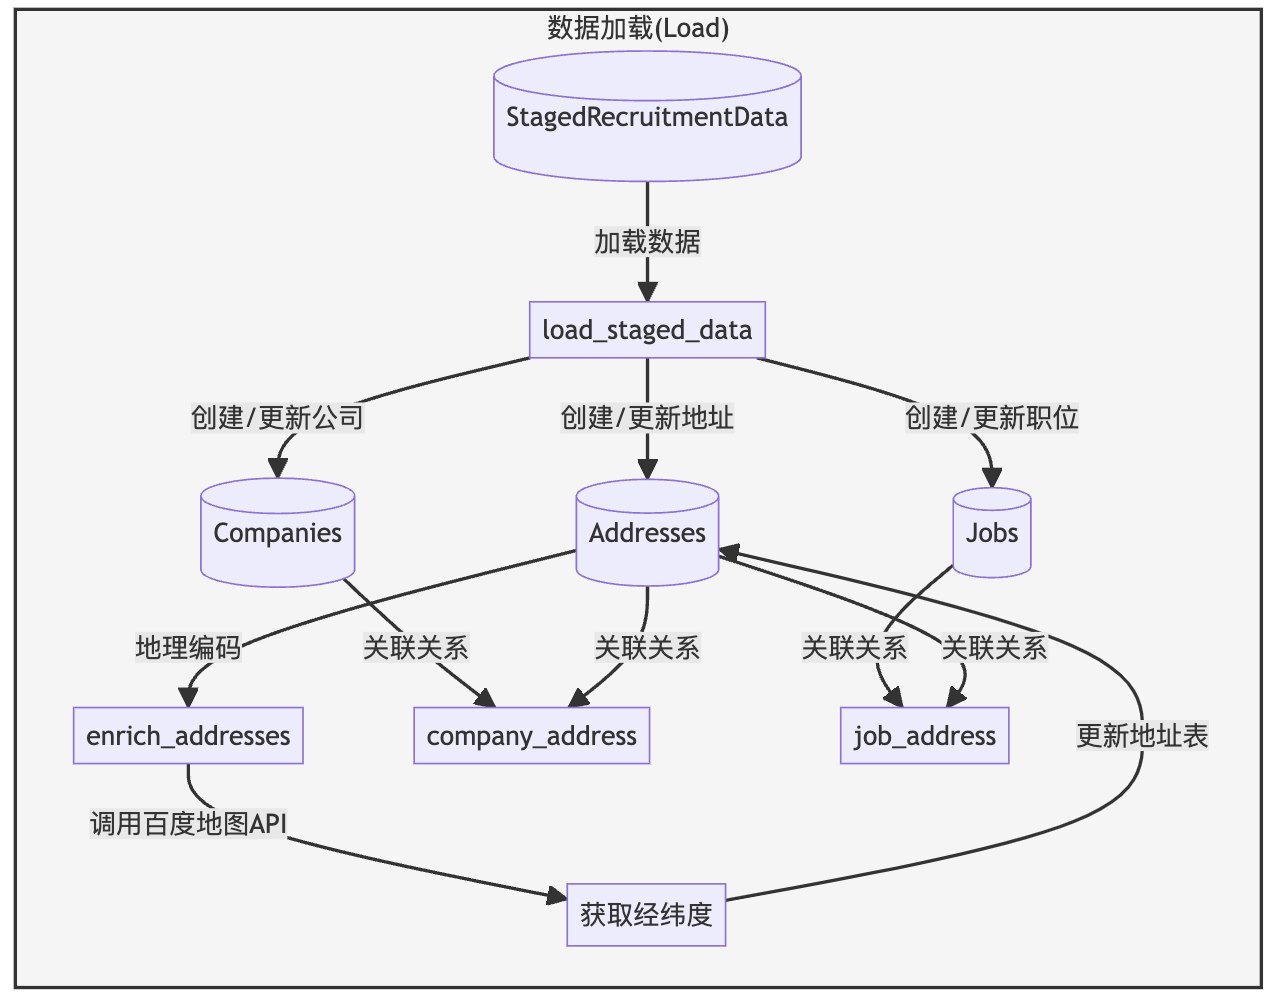
\includegraphics[width=0.5\textwidth]{figures/load.png}
    \caption{ETL数据加载流程}
    \label{fig:ETL_load}
\end{figure}

\subsubsection{CRUD层}
CRUD层作为系统的数据访问中间层,提供了统一的数据操作接口。该层的设计遵循了领域驱动设计(DDD)的原则,将业务逻辑与数据访问清晰分离:

\begin{itemize}
    \item \textbf{数据读取模块}:
    \begin{itemize}
        \item 职位数据读取:实现了高效的职位信息检索,支持多条件组合查询
        \item 公司数据读取:提供完整的公司信息访问接口,支持模糊匹配和精确查询
        \item 薪资数据读取:实现了复杂的薪资统计算法,支持多维度的薪资分析
        \item 地理数据读取:提供基于地理位置的数据检索,支持范围查询和距离计算
    \end{itemize}
    
    \item \textbf{数据解析模块}:
    \begin{itemize}
        \item 薪资解析器:采用智能算法解析多种格式的薪资描述,实现标准化处理
        \item 地址解析器:结合百度地图API,实现精确的地址解析和地理编码
        \item 数据转换解析器:提供灵活的数据转换框架,支持自定义转换规则
    \end{itemize}
    
    \item \textbf{物化视图管理}:
    \begin{itemize}
        \item 实现了智能的视图更新策略,根据数据变化频率动态调整更新周期
        \item 提供了完整的视图管理接口,支持视图的创建、更新和删除
        \item 实现了视图依赖管理,确保相关视图的同步更新
    \end{itemize}
\end{itemize}

\subsection{前端实现}

本系统的前端采用现代化的Web开发技术栈,基于采用文件路由系统的Next.js 15框架构建.


如前端项目的组件关系图\ref{fig:front_end_structure}所示,系统采用了基于Next.js的分层设计,从配置层(config.ts、globals.css、fonts.ts)到导航布局(layout.tsx)再到具体的功能页面(MapPage、FilterPage、OverviewPage)。每个功能页面都对应特定的数据可视化组件(MapPlot、FilterPlot、OverviewPlot),这些组件分别使用了不同的可视化库(Plotly.js Map、NextUI组件、Plotly.js Charts和Dashboard)来实现地图展示、数据筛选和统计概览等功能。整个前端架构通过统一的API调用(salary-distribution、filter-data、overview-stats)与后端进行数据交互,实现了清晰的数据流动和模块化的功能划分。

\begin{figure}[htbp]
    \centering
    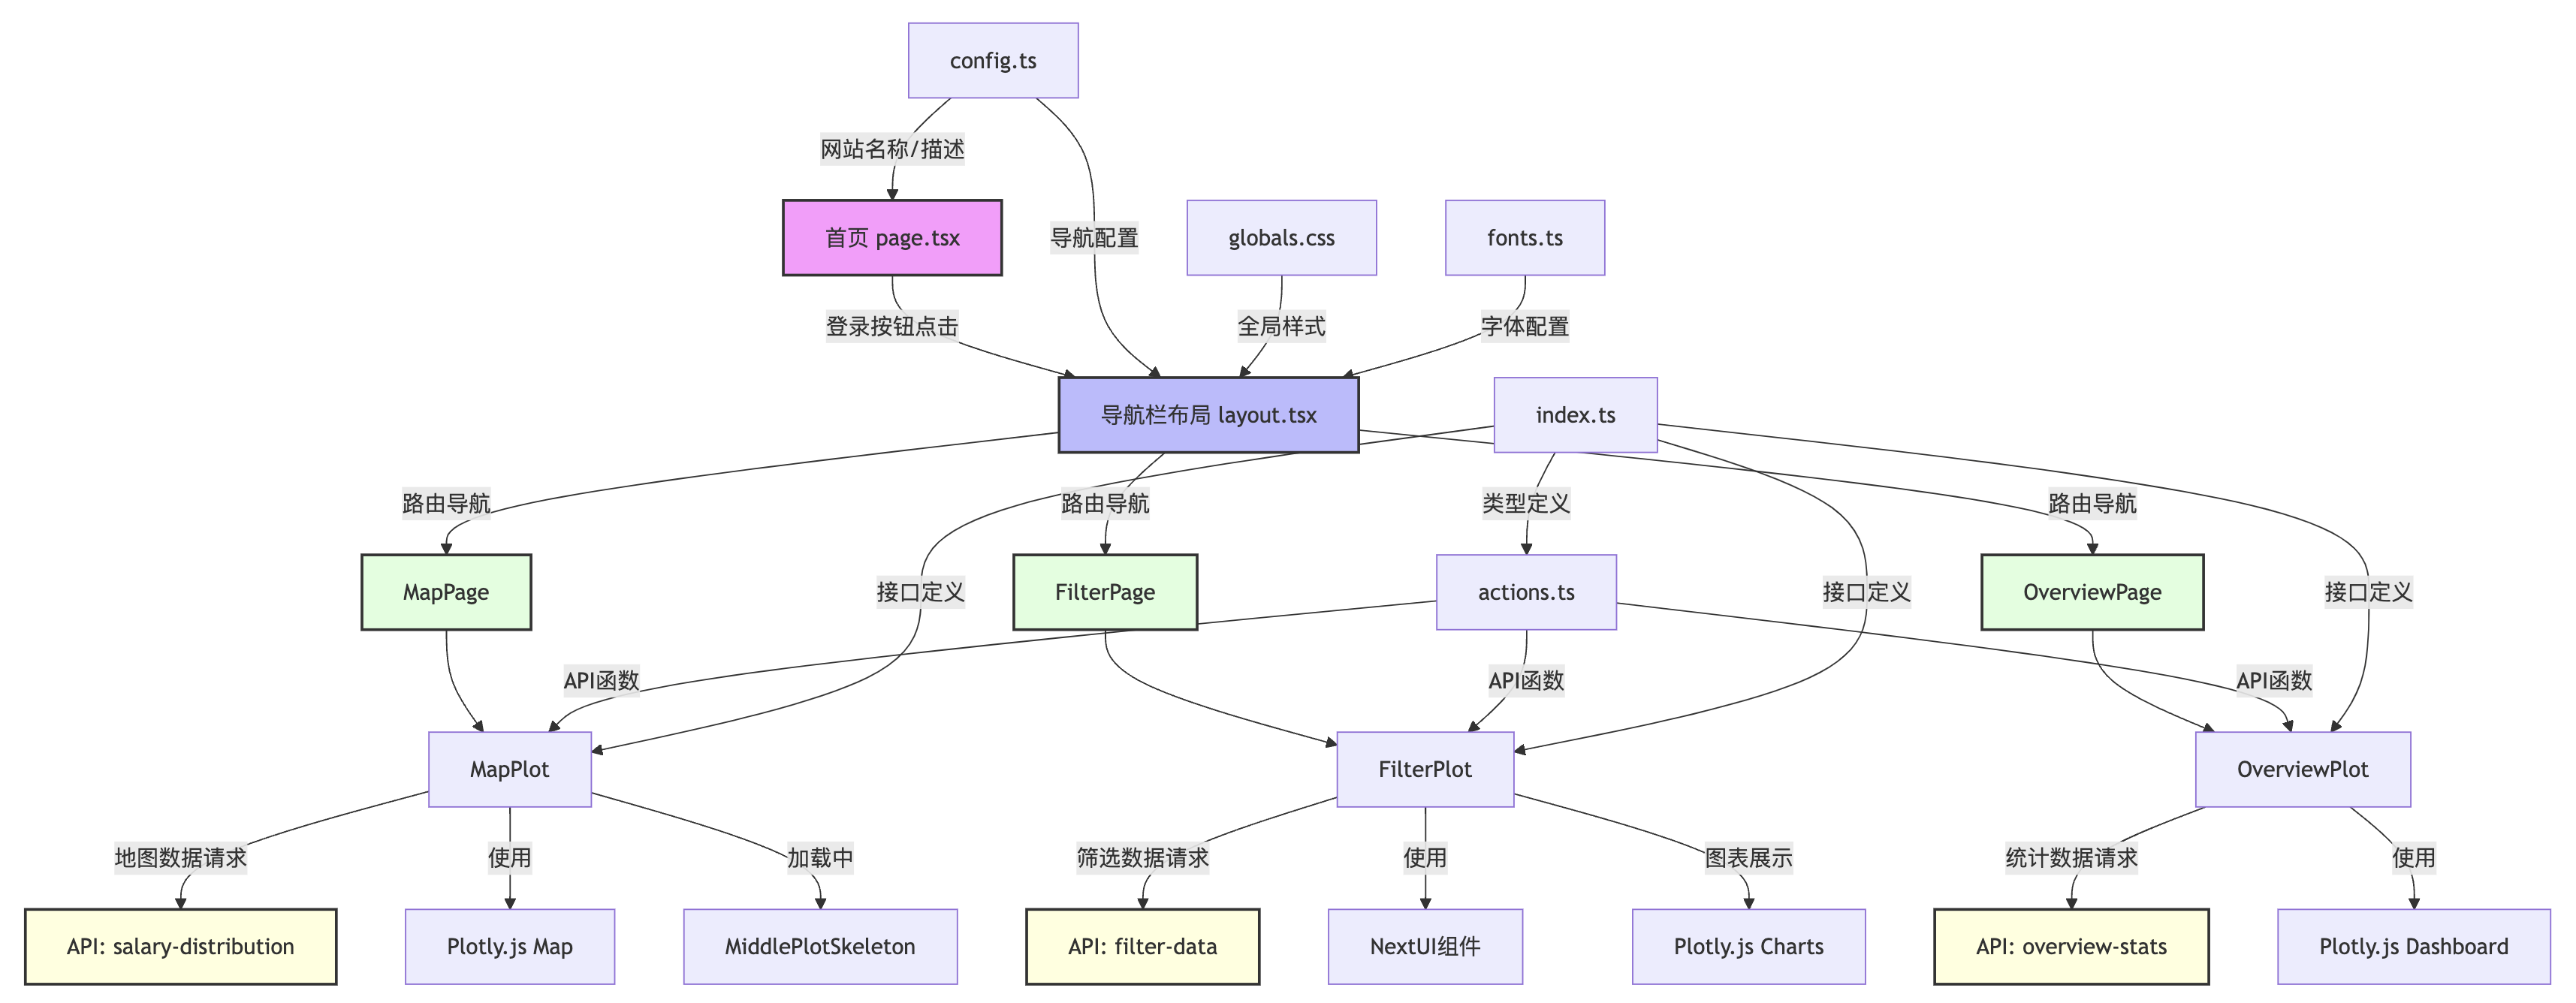
\includegraphics[width=1.0\textwidth]{figures/前端项目结构图.png}
    \caption{前端项目结构图}
    \label{fig:front_end_structure}
\end{figure}

如前端数据流图\ref{fig:front_end_data_flow}所示,系统采用了基于React Hooks的状态管理模式,从用户交互(用户点击、用户输入、用户选择)开始,通过useState和useEffect等钩子函数管理状态和副作用。数据流经过actions.ts进行统一的动作处理,然后通过fetch请求调用后端API。获取的数据经过数据解析和TypeScript类型转换后,最终通过Plotly.js或NextUI组件进行可视化展示,同时系统还实现了错误处理和加载状态显示,形成了一个完整的前端数据处理闭环。这种设计保证了数据流的单向性和可预测性,提高了应用的可维护性和性能。


\begin{figure}[htbp]
    \centering
    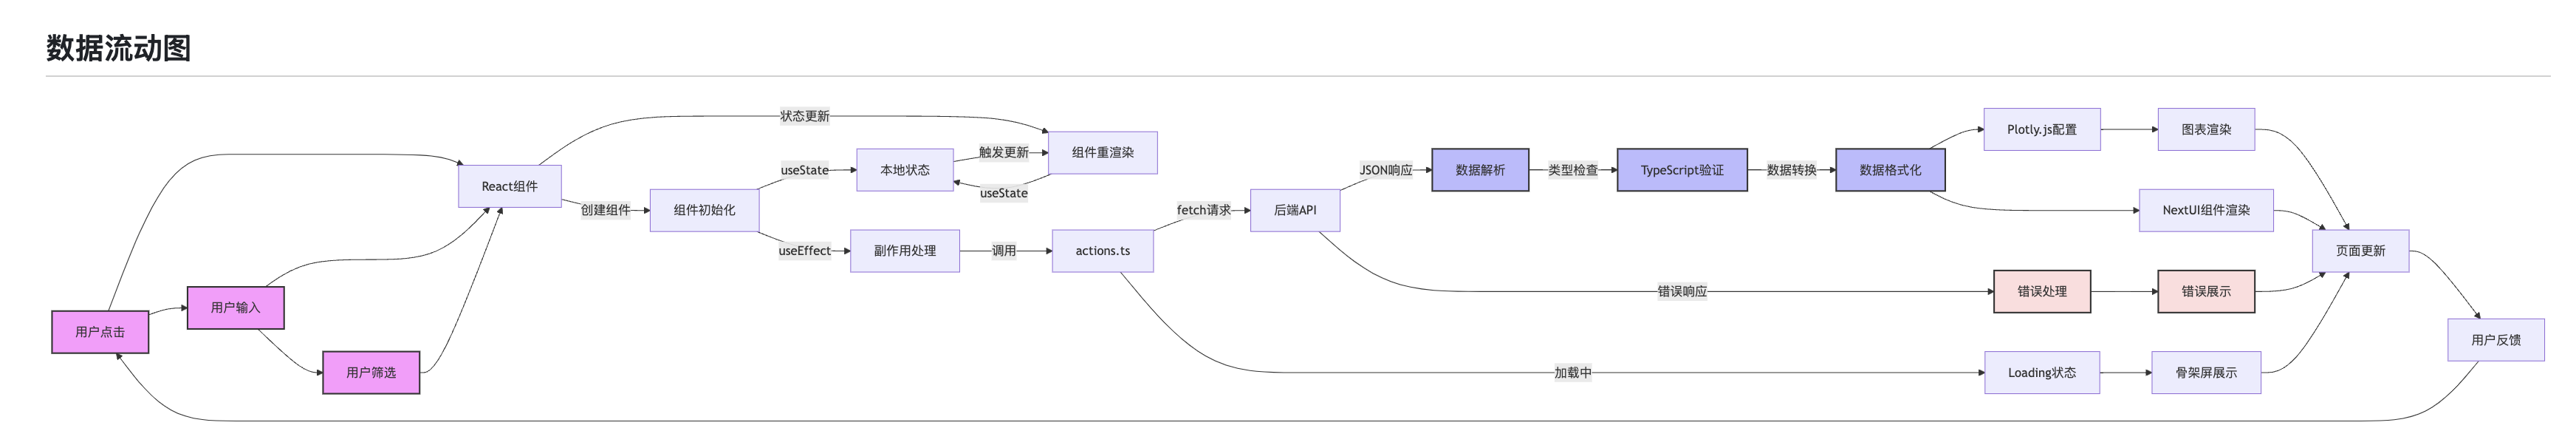
\includegraphics[width=1.0\textwidth]{figures/前端数据流图.png}
    \caption{前端数据流图}
    \label{fig:front_end_data_flow}
\end{figure}

